% Paper draft (ACL ARR long-paper template, 3,000-4,000 words). Skeleton only: section headings and figure slots.
% Build: python make_figures.py && pdflatex main && bibtex main && pdflatex main && pdflatex main
\documentclass[11pt]{article}
\usepackage[review]{acl}            % review = anonymous; preprint = names and page numbers (for the supervisor copy)
\usepackage{times}
\usepackage{latexsym}
\usepackage[T1]{fontenc}
\usepackage[utf8]{inputenc}
\usepackage{microtype}
\usepackage{graphicx}
\usepackage{booktabs}

\title{Riding the Wave? Tradition and Innovation in Machine Learning Research\\during the Foundation-Model Shift}
\author{Minghan Li \\ Supervisor: A/Prof Jianzhong Qi}

\begin{document}
\maketitle

\begin{abstract}
% Part 1
\end{abstract}

\section{Introduction}
% Part 1

\section{Background: The Essential Tension}
% Part 3

\section{Data, Measurement and Evidence Tiers}
% Part 3

\section{The Field: Waves, Seen without Hindsight}
% Part 2
\begin{figure*}[t]
  \centering
  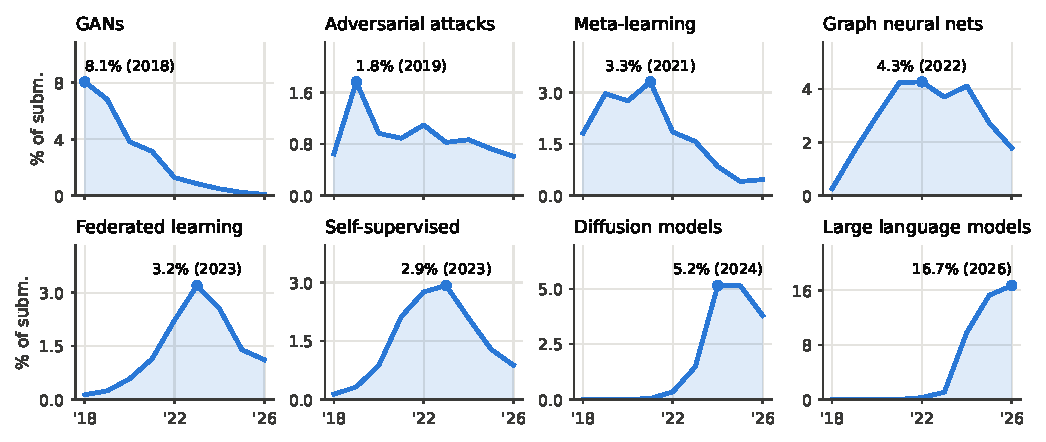
\includegraphics[width=\textwidth]{figs/fig1_waves.pdf}
  \caption{Research waves at ICLR: share of submissions listing each author keyword, 2018--2026 (peak marked).}
  \label{fig:waves}
\end{figure*}

\section{People: Who Brings the New}
% Part 2

\section{Review: What Is Rewarded}
% Part 2

\section{Discussion}
% Part 3

\section{Conclusion}
% Part 3

\section*{Limitations}
% Part 3 (required by ARR; not counted in the page limit)

\bibliography{references}

\appendix
\section{Appendix}
% Part 3

\end{document}
